\begin{savequote}[8cm]
Conoscere nel senso della Scienza vuol dire prevedere.

To know in its Scientific meaning, means to predict.
  \qauthor{--- Carlo Rubbia}
\end{savequote}

\chapter{\label{ch:3-DUNE}The Deep Underground Neutrino Experiment}


\minitoc
\section{Introduction} \label{ch3-Sec:Introduction}
\begin{figure}[!ht]
     \centering
     \includegraphics[width=0.99\textwidth]{figures/ch3-DUNE/LBNE_Graphic_061615_2016.jpg}
     \caption{Schematic representation of the DUNE experiment with its main components}
        \label{fig:DUNEdiagram}
\end{figure}
The Deep Underground Neutrino Experiment (DUNE) will be a next generation long baseline neutrino oscillation experiment \cite{DUNE:2020TDR1}. Its main goal will be to measure all the parameters governing neutrino and anti-neutrino oscillations in a single experiment, with particular emphasis on the CP violation phase $\delta_\textrm{CP}$ and the neutrino mass ordering. The experiment will consist of three main components: a wide band high intensity neutrino beam situated at Fermilab, which will be capable of producing both a $\nu_\mu$ and a $\Bar{\nu}_\mu$ fluxes; a kt-scale underground liquid Argon based Far Detector (FD), situated at the Sanford Underground Research Facility (SURF) in South Dakota, at $\sim1300$ Km from the source; a modular Near Detector (ND) situated at $\sim500$ m from the source.

Due to budgetary restrictions DUNE will pursue a staged approach in its construction and data production \cite{DUNE:2022Snowmass}. The initial composition of the experiment, referred to as Phase I, will include two LArTPC Far Detector modules, both being 10kt in volume, but utilizing a Vertical Drift \cite{DUNE:2023TDRVD} and an Horizontal Drift (or Single Phase) technology \cite{DUNE:2020TDR4} respectively. The initial configuration of the ND will include two out of the three originally envisioned detectors: the liquid argon near detector ND-LAr, a modular LArTPC similar in technology to the FD modules and the system for on axis neutrino detection SAND, whose main function will be to act as a beam monitor \cite{Battisti:2022ND}. A third ND module will be placed between ND-LAr and SAND to act as a muon spectrometer: this will be called the Temporary Muon Spectrometer (TMS) and will be removed from the ND facilities after Phase I to be replaced by a more capable detector. In Phase I DUNE will be able to determine the neutrino mass ordering, measure $\delta_\textrm{CP}$ at 3$\sigma$ if maximal, measure several oscillation parameters at world-leading levels of precision, detect supernova collapse neutrinos if available and search for BSM physics. 

In order to pursue its full physics scope, after Phase I DUNE will undertake several key improvements to all of its key components: this second form of the experiment is referred to as Phase II. The Far Detector will be completed by two extra liquid argon modules (nominally using the Verdical Drift technology) for a total fiducial mass of at least 40kt. The proton beam's power will augmented from 1.2 MW to 2.4 MW. The TMS will be replaced by a more capable high pressure gaseous Argon magnetized detector called ND-GAr. All of these upgrades are necessary for DUNE to reach one of its key stated goals: reach 5$\sigma$ sensitivity on CP violation over a wide range of $\delta_\textrm{CP}$ values. Additionally in Phase II, DUNE will be capable of producing independent measurements of $\sin^2{\theta_{13}}$ with precision comparable to that of reactors, it will have significant sensitivity to the $\theta_{23}$ octant, and will reach a world-leading sensitivity in a wide range of physics beyond the three neutrino paradigm as well as additional BSM physics and astrophysics. 

\section{DUNE's facilities and design}
In this section we give a brief overview of the components constituting the DUNE experiment, including the neutrino beamline, the Near Detector and the Far Detector. The muon spectrometer component of the Near Detector, which includes the ND-GAr detector for Phase I and the temporary muon spectrometer for Phase II, will be discussed in more detail in dedicated sections as they constitute the main focus of this thesis.


\subsection{The LBNF beamline}
\begin{figure}[!h]
     \centering
     \includegraphics[width=0.99\textwidth]{figures/ch3-DUNE/LBNF-IL-graphic-Fermilab-LBNF.png}
     \caption{Schematic representation of the DUNE experiment with its main components}
        \label{fig:KFdiagram}
\end{figure}
The neutrino flux that will be utilized by the DUNE experiment, will be produced by the LBNF Beamline at Fermilab, which is expected to produce the highest power neutrino beam in the world \cite{DUNE:2016LBNFTDR, Papadimitriou:2016ksv}. The production of the neutrino flux begins by accelerating protons through a proton accelerator. The primary proton beam, which operates in the energy range of 60-120 GeV, is extracted from Fermilab's Main Injector (MI), a proton accelerator already utilized by the NOvA experiment and partially based on the Tevatron collider facilities. The main injector will be upgraded through the Proton Improvement Plan, phase II (PIP-II), in time for the DUNE Phase I data taking period to reach average beam powers of the order of 1.14 MW, delivering $7.5 \times 10^{13}$ protons in one MI machine cycle (0.7 sec - 1.2 sec) to the LBNF target. Further improvements are expected the PIP III project to reach 2.4 MW of power for DUNE Phase II and all the beamline components are being planned to accommodate these improvements with minimal retro-fitting. 

Once the primary proton beam reaches the desired energy, it is directed through the use of extraction and transport components over a man-made hill and bent downwards towards a graphite target located at grade level. This constitutes the first element of the proper neutrino beamline. The charged mesons, primarily kaons and pions, produced in the interactions of the protons are sign selected and focused by two magnetic horns into a decay pipe toward the far detector. The target and focusing horns are all located inside a heavily shielded vault called the target chase, that is isolated from the decay pipe at its downstream end by a metallic window. Their design is derived from that of the NuMi neutrino beam. 

The mesons produced in the proton interactions are short-lived and decay into either anti-muons and neutrinos or muons and anti-neutrino,s depending on the charge of the mesons. If the main neutrino types being produced are $\nu_\mu$ the Beamline is said to be in Forward Horn Current (FHC) mode, otherwise it is said to be in Reverse Horn Current (RHC) mode.  Both polarities will produced high purity
fluxes, with an expected contamination from the “incorrect” neutrino type (i.e. $\nu_\mu$ in RHC mode and vice-versa) of less than 10\% in the oscillation energy region. This type of impurities are introduced by hadrons of the opposite sign propagating at the centre of the beam, where no magnetic field is present. A small $\nu_e$ and $\Bar{\nu}_e$
component is also introduced by the decay of secondary kaons and tertiary muons from pion decays. At the end of the decay region, an absorber is needed to remove the residual hadrons remaining at the end of the decay pipe.  The absorber core consists of replaceable aluminium and steel water-cooled blocks. Approximately 40\% of the beam power is deposited in the target chase and surrounding shielding, 30\% in the decay pipe and 30\% in the absorber.

The wide band neutrino beam which is produced by the Beamline facilities, is needed to cover the first and second neutrino oscillation maxima, which for a 1300 km baseline are expected to be approximately at 2.4 and 0.8 GeV. For this reason the beamline design is optimized for neutrino energies between 0.5 and 5 GeV. 

\subsection{The Far Detector}
\begin{figure}[!ht]
     \centering
     \includegraphics[width=0.99\textwidth]{figures/ch3-DUNE/Far_Detector.jpg}
     \caption{Schematic representation of the Far Detector experiment with its main components}
        \label{fig:FarDetectorHall}
\end{figure}
The DUNE Far Detector will be composed of four LArTPC detector module, each containing a 10kt fiducial liquid Argon mass  and a total liquid Argon mass of 17.5kt. Each module will fit inside a cryostat. Of the four modules only the first two will be available during DUNE Phase I, the first one using an Horizontal Drift technology (originally identified as Single Phase \cite{DUNE:2020TDR4}) will be called FD1-HD and the second one using a Vertical Drift technology\cite{DUNE:2023TDRVD} (evolved from the Dual Phase Technology \cite{DUNE:2018mlo}) will be called FD2-VD. The last two modules will be employed during Phase II and are nominally set to be Vertical Drift detectors\cite{DUNE:2022Snowmass}.

The LArTPC was pioneered by the ICARUS experiment \cite{Rubbia:1977zz,ICARUS:2004wqc} and is now a mature detector technology within the neutrino experiment community, being employed in detectors such as MicroBooNe\cite{MicroBooNE:2016pwy} and SBND\cite{Machado:2019oxb} at Fermilab as well as the ProtoDUNE-SP\cite{DUNE:2020cqd} prototype tested at the CERN neutrino facilities. In a LArTPC, ionization electrons produced by the energy deposition of charged particles generated in neutrino interactions, are drifted by an electric field in the liquid Argon towards an anode and are collected on a charge multiplier element, producing a readable two dimensional signal. The measurement of the collected ionization electrons also provides a measurement of the $dE/dx$ of the charged particles, which is what enables both calorimetry and particle identification (PID) in a LArTPC.

Argon is a UV light scintillator. Once shifted into the visible spectrum, the UV scintillation photons produced by can be collected by photon detectors and provide an initial start time $t_0$, indicating when the ionization electrons begin to drift. Comparing the time at which the ionization signal reaches the anode relative to this start time allows reconstruction of the event topology in the drift coordinate. 

The FD1-HD design combines a kt level fiducial mass with a sub-cm spacial resolution. Both are crucial to achieve DUNE's scientific goals of measuring CP violation, while searching for nucleon decay and being capable of observing neutrinos from supernova bursts. An example of the design of the detector being directly informed by the physics requirements of the experiment, comes from the electron/photon separation requirements necessary to study $\nu_e$ appearance signals in the LBNF $\nu_\mu$ flux. Electrons are typically produced in charged current $\nu_e$ interactions and induce electro-magnetic showers in the LAr medium. Similar electro-magnetic activity can be induced by photons coming for example from $\pi^0$ decay. The FD modules are capable of distinguishing between these two signals by using $dE/dx$ information combined with spacial information. Photon induced signals have an initial non ionized gap of several cm's before the formation of the electro-magnetic shower and have a $dE/dx$ which is double that of an electron induced one.

\begin{figure}[!t]
     \centering
     \includegraphics[width=0.8\textwidth]{figures/ch3-DUNE/TheBoPicture.png}
     \caption{Schematic representation of the Far Detector experiment with its main components}
        \label{fig:LArTPCdiagram}
\end{figure}

The FD1-HD detector modules consist of 4 separate liquid Argon filled drift volumes with a maximum drift length of 3.5 m. Each Volume is instrumented with a vertical cathode plane and an anode plane, for a total of three module-long (58.2 m) anode planes and two cathode planes. A field cage covers the spaces between the two, producing a stable 500 V/m electric field in the horizontal direction. The drift ionization electrons reach the anode planes in an order of a few milli-seconds. 

Each anode plane is instrumented with a total of 50 anode plane assemblies APAs which consist of an aluminum frame with three layers of active wires and an additional shielding layer wrapped around them. The first two active layers are identified as the U and V induction layers. These layers are angled at a $\pm 37.5^\circ$ in order to reduce ambiguities in event reconstruction. The relative voltage between the layers is chosen so that the drift electrons pass through them and produce a bipolar induction signal on both planes. The drifting electrons are finally collected in the final $X$ wire plane, where they produce a mono-polar signal. In the $X$ collection plane, as well as in the $G$ shielding plane, the wires run vertically. The spacing between the wires in each layer is of 5 mm, and defines the spacial resolution of the APAs.

The scintillation photons produced by the passing charged particles in the liquid Argon in the very ultra violet (VUV) spectrum are collected by photon detector (PD) systems called X-ARAPUCA \cite{Segreto:2018jdx}. The photons are produce in the order of 24000 per MeV of deposited energy, and reach the detectors in a time-frame of the order of a nanosecond. The X-ARAPUCA modules are mounted between the sets of wire-planes and consist of layers of dichroic filter and wavelength shifters, that shift the VUV scintillation light into the visible range, trap the visible photons, and transport them to a silicon photo-multiplier (SiPM). The signals produced in the SiPMs are then combined with the wire signals from the APAs at the data acquisition (DAQ) level.

\begin{figure}[!t]
     \centering
     \includegraphics[width=0.7\textwidth]{figures/ch3-DUNE/setup_new_updated.png}
     \caption{Schematic representation of the Far Detector experiment with its main components}
        \label{fig:FDLArTPCModule}
\end{figure}

The FD2-VD design has developed from the R\&D experience accumulated by the DUNE collaboration with the ProtoDUNE-SP and ProtoDUNE-DP prototypes at the neutrino research facilities at CERN. The detector consists of several vertical drift modules enclosed in a large cryostat structure. Each module is divided into two vertical drift regions 6.5 m in height, by an horizontal cathode and feature two anode planes, one close to the cryostat top, just below the surface of the liquid Argon region and one close to the bottom of the cryostat. Field cage modules hang vertically around the module's perimeter. The 450 V/cm electric field drifts the ionisation electrons, either upwards or downwards depending on the drift region. The vertical design of the FD2-VD offers a slightly larger instrumented module compared to FD1-HD and it's more cost-effective thanks to its high-modularity and general structure and geometry. 

The anode planes in the FD2-VD design consist of two double-sided perforated printed circuit boards (PCBs) that are connected to form a charge-readout unit (CRUs). The perforation holes allow the electrons to pass through the PCB's. The first PCB is instrumented with two sets of induction strips, while the second one hosts the collection strips. The three planes of strips are segmented at about 7.5 mm pitch for the induction planes and 5 mm pitch for the collection plane, and are set at $60^\circ$ angles relative to each other to maximize information in the charge readout from different projections. Two CRU's are connected to a frame to form a Charge Readout Plane (CRP). Each anode plane consists of 80 CRP's. Much like in the FD1-HD design the anode plane signal allows for a two-dimensional reconstruction of any given event, while the third dimension is given by the drift time information obtained from the scintillation light.

The PD's implemented in the FD2-VD follow the same general design of the ARAPUCA-X modules developed for FD1-HD. The PDs will be mounted on the four cryostat membrane walls as on both sides of the central cathode structure. This configuration offers a uniform ligth measurement coverage across the entire LArTPC volume. Additionally, the FD2-VD liquid argon will be doped with a small quantity of xenon. This has no impact on the TPC operation but significantly enhances the photon detection performance.

\subsection{The Near Detector}

\begin{figure}[!h]
     \centering
     \includegraphics[width=0.99\textwidth]{figures/ch3-DUNE/ndhall.JPG}
     \caption{Schematic representation of the Far Detector experiment with its main components}
        \label{fig:NDhall}
\end{figure}

To enable oscillation measurements, DUNE must first predict the anticipated signal and background at the Far Detector based on oscillation parameters, followed by a comparison with measured flavour-tagged neutrino spectra. To generate this prediction, one must determine the neutrino flux at production, neutrino interaction cross-sections, and detector response—factors all affected by systematic uncertainties requiring constraint. The Near Detector (ND) is tailored to address each prediction component \cite{DUNE:2021NDCDR}: it will gauge the un-oscillated neutrino beam flux both on-axis and at varying off-axis angles; refine models of neutrino interactions through cross-section and final state topology measurements; model detector responses relative to neutrino energy. Additionally, the ND is designed for operation within a high event rate environment, ensuring the requisite statistical coverage across the full phase-space. The ND will be of three detectors with complementary designs: ND-LAr, which will use a LArTPC technology similar to the FD modules; ND-GAr, a gaseous Argon TPC detector; and SAND, a magnetized beam monitor. ND-LAr and ND-GAr are movable off-axis and will contribute to the DUNE-PRISM program, while SAND remains fixed on-axis. A schematic depiction of the Near Detector, inclusive of all detectors, is presented in Figure \ref{fig:NDhall}. Due to budgetary reasons the ND-GAr detector will become available only during Phase II of the DUNE experiment. A much simpler detector referred to as the Temporary Muon Spectrometer (TMS) will replace it during Phase I. Both ND-GAr and the TMS will be discussed in a dedicated section along-side an alternative and now abandoned Phase I muon spectrometer design called ND-GAr-Lite. 


\begin{figure}[!t]
     \centering
     \begin{subfigure}[b]{0.59\textwidth}
         \centering
         \includegraphics[width=\textwidth]{figures/ch3-DUNE/ND-LAr.jpg}
         \caption{}
         \label{fig:NDLAr}
     \end{subfigure}
     \begin{subfigure}[b]{0.39\textwidth}
         \centering
         \includegraphics[width=\textwidth]{figures/ch3-DUNE/ND-LAr_module.png}
         \caption{}
         \label{fig:NDLArModule}
     \end{subfigure}
        \caption{(a) Average $\beta$ as a function of the track length $l $ and  (b) average track length as a function of the true momentum $p_\textrm{true}$ for the HP sample.}
        \label{fig:ND-Larview}
\end{figure}

ND-LAr is a LArTPC detector engineered for operation within a high-rate environment. Utilizing the same Argon target and similar detector technology as the FD modules, ND-LAr is essential for modeling detector response and liquid Argon neutrino interaction cross-sections. ND-LAr is comprised of 35 distinct TPC modules, mirroring the design of the ArgonCube prototype \cite{Dwyer:2018phu}. Despite the relativly modest dimentions of the detector, this modular architecture is indispensable for managing the high event rate, facilitating a smaller drift region, enhanced light separation, and increased sensor pixelation. Each module encompasses two optically isolated TPCs outfitted with a LArPix-based pixelated charge readout system  \cite{Goldi:2018mbo}, alongside a light readout for rapid timing data from prompt scintillation light, and a field structure ensuring minimal field non-uniformity throughout the active volume. Given the relatively compact dimensions of its active volume, ND-LAr cannot fully contain the majority of muons generated in $\nu_\mu$ Charged Current (CC) interactions within liquid Argon. Hence, precise momentum reconstruction of this muon sample necessitates an external spectrometer component, a role fulfilled by ND-GAr and the TMS.

\begin{figure}[t]
     \centering
     \begin{subfigure}[b]{0.5\textwidth}
         \centering
         \includegraphics[width=\textwidth]{figures/ch3-DUNE/SAND.png}
         \caption{}
         \label{fig:SAND-outside}
     \end{subfigure}
     \hfill
     \begin{subfigure}[b]{0.48\textwidth}
         \centering
         \includegraphics[width=\textwidth]{figures/ch3-DUNE/SAND-inside.png}
         \caption{}
         \label{fig:SAND-inside}
     \end{subfigure}
        \caption{(a) Schematic view of the external components of SAND, including its cryostat and its solenoid magnet (b) Side view of the internal components of SAND, including its active liquid Argon target called GRAIN, one of the straw tube tracker modules and the electro-magnetic calorimeter.  }
        \label{fig:SAND-all}
\end{figure}

ND-LAr and ND-GAr possess the capability to be translated up to 30 meters perpendicular to the neutrino beam axis, spanning angles from $0^{\circ}$ to $3^{\circ}$, a feature named DUNE-PRISM. With increasing off-axis angles, the mean energy of the neutrino flux diminishes while its energy dispersion narrows. Consequently, the Near Detector gains access to diverse un-oscillated neutrino flux profiles, combining them to predict the oscillated flux at the far detector. This data-centric methodology mitigates reliance on models. Moreover, a key feature of the DUNE-PRISM program is that the off-axis fluxes will variate in mean energies and spreads and will thus be dominated by distinct interaction types (e.g., quasi-elastic, resonant etc.). Access to this variety of samples will facilitate the disentanglement of cross-section effects, enhancing flux and interaction modeling.

The System for On-Axis Neutrino Detection (SAND) will function as a constant on-axis monitor of the neutrino beam, a crucial role for the DUNE-PRISM program. It will ensure that any differences in flux measured by ND-LAr and ND-GAr result from their off-axis position rather than anomalies in beam production. SAND's main structural components, along with its solenoid magnet, cryostat, and electromagnetic calorimeter, will be repurposed from the KLOE experiment (Figure \ref{fig:SAND-all}). The internal tracker design of SAND has recently been finalized, featuring a Straw Tube Tracker (STT) divided in modules. These modules will include a series of tunable passive slabs interleaved with tracking layers of 5mm diameter tubes. SAND will provide various targets, such as CH$_2$ and C, potentially highly useful in studying neutrino interactions. They will offer a clean sample of neutrino-on-hydrogen interactions by "subtraction," devoid of nuclear effects. Additionally, SAND will incorporate its own active target of liquid Argon called GRAIN, whose design is currently being finalized. 

\section{The ND-GAr detector}
\label{sec:DUNE-ND-GAr}
% \begin{figure}
%      \centering
%      \begin{subfigure}[b]{0.4\textwidth}
%          \centering
%          \includegraphics[width=\textwidth]{figures/ch3-DUNE/ND_GAr.jpg}
%          \caption{}
%          \label{fig:ND-G}
%      \end{subfigure}
%      \hfill
%      \begin{subfigure}[b]{0.58\textwidth}
%          \centering
%          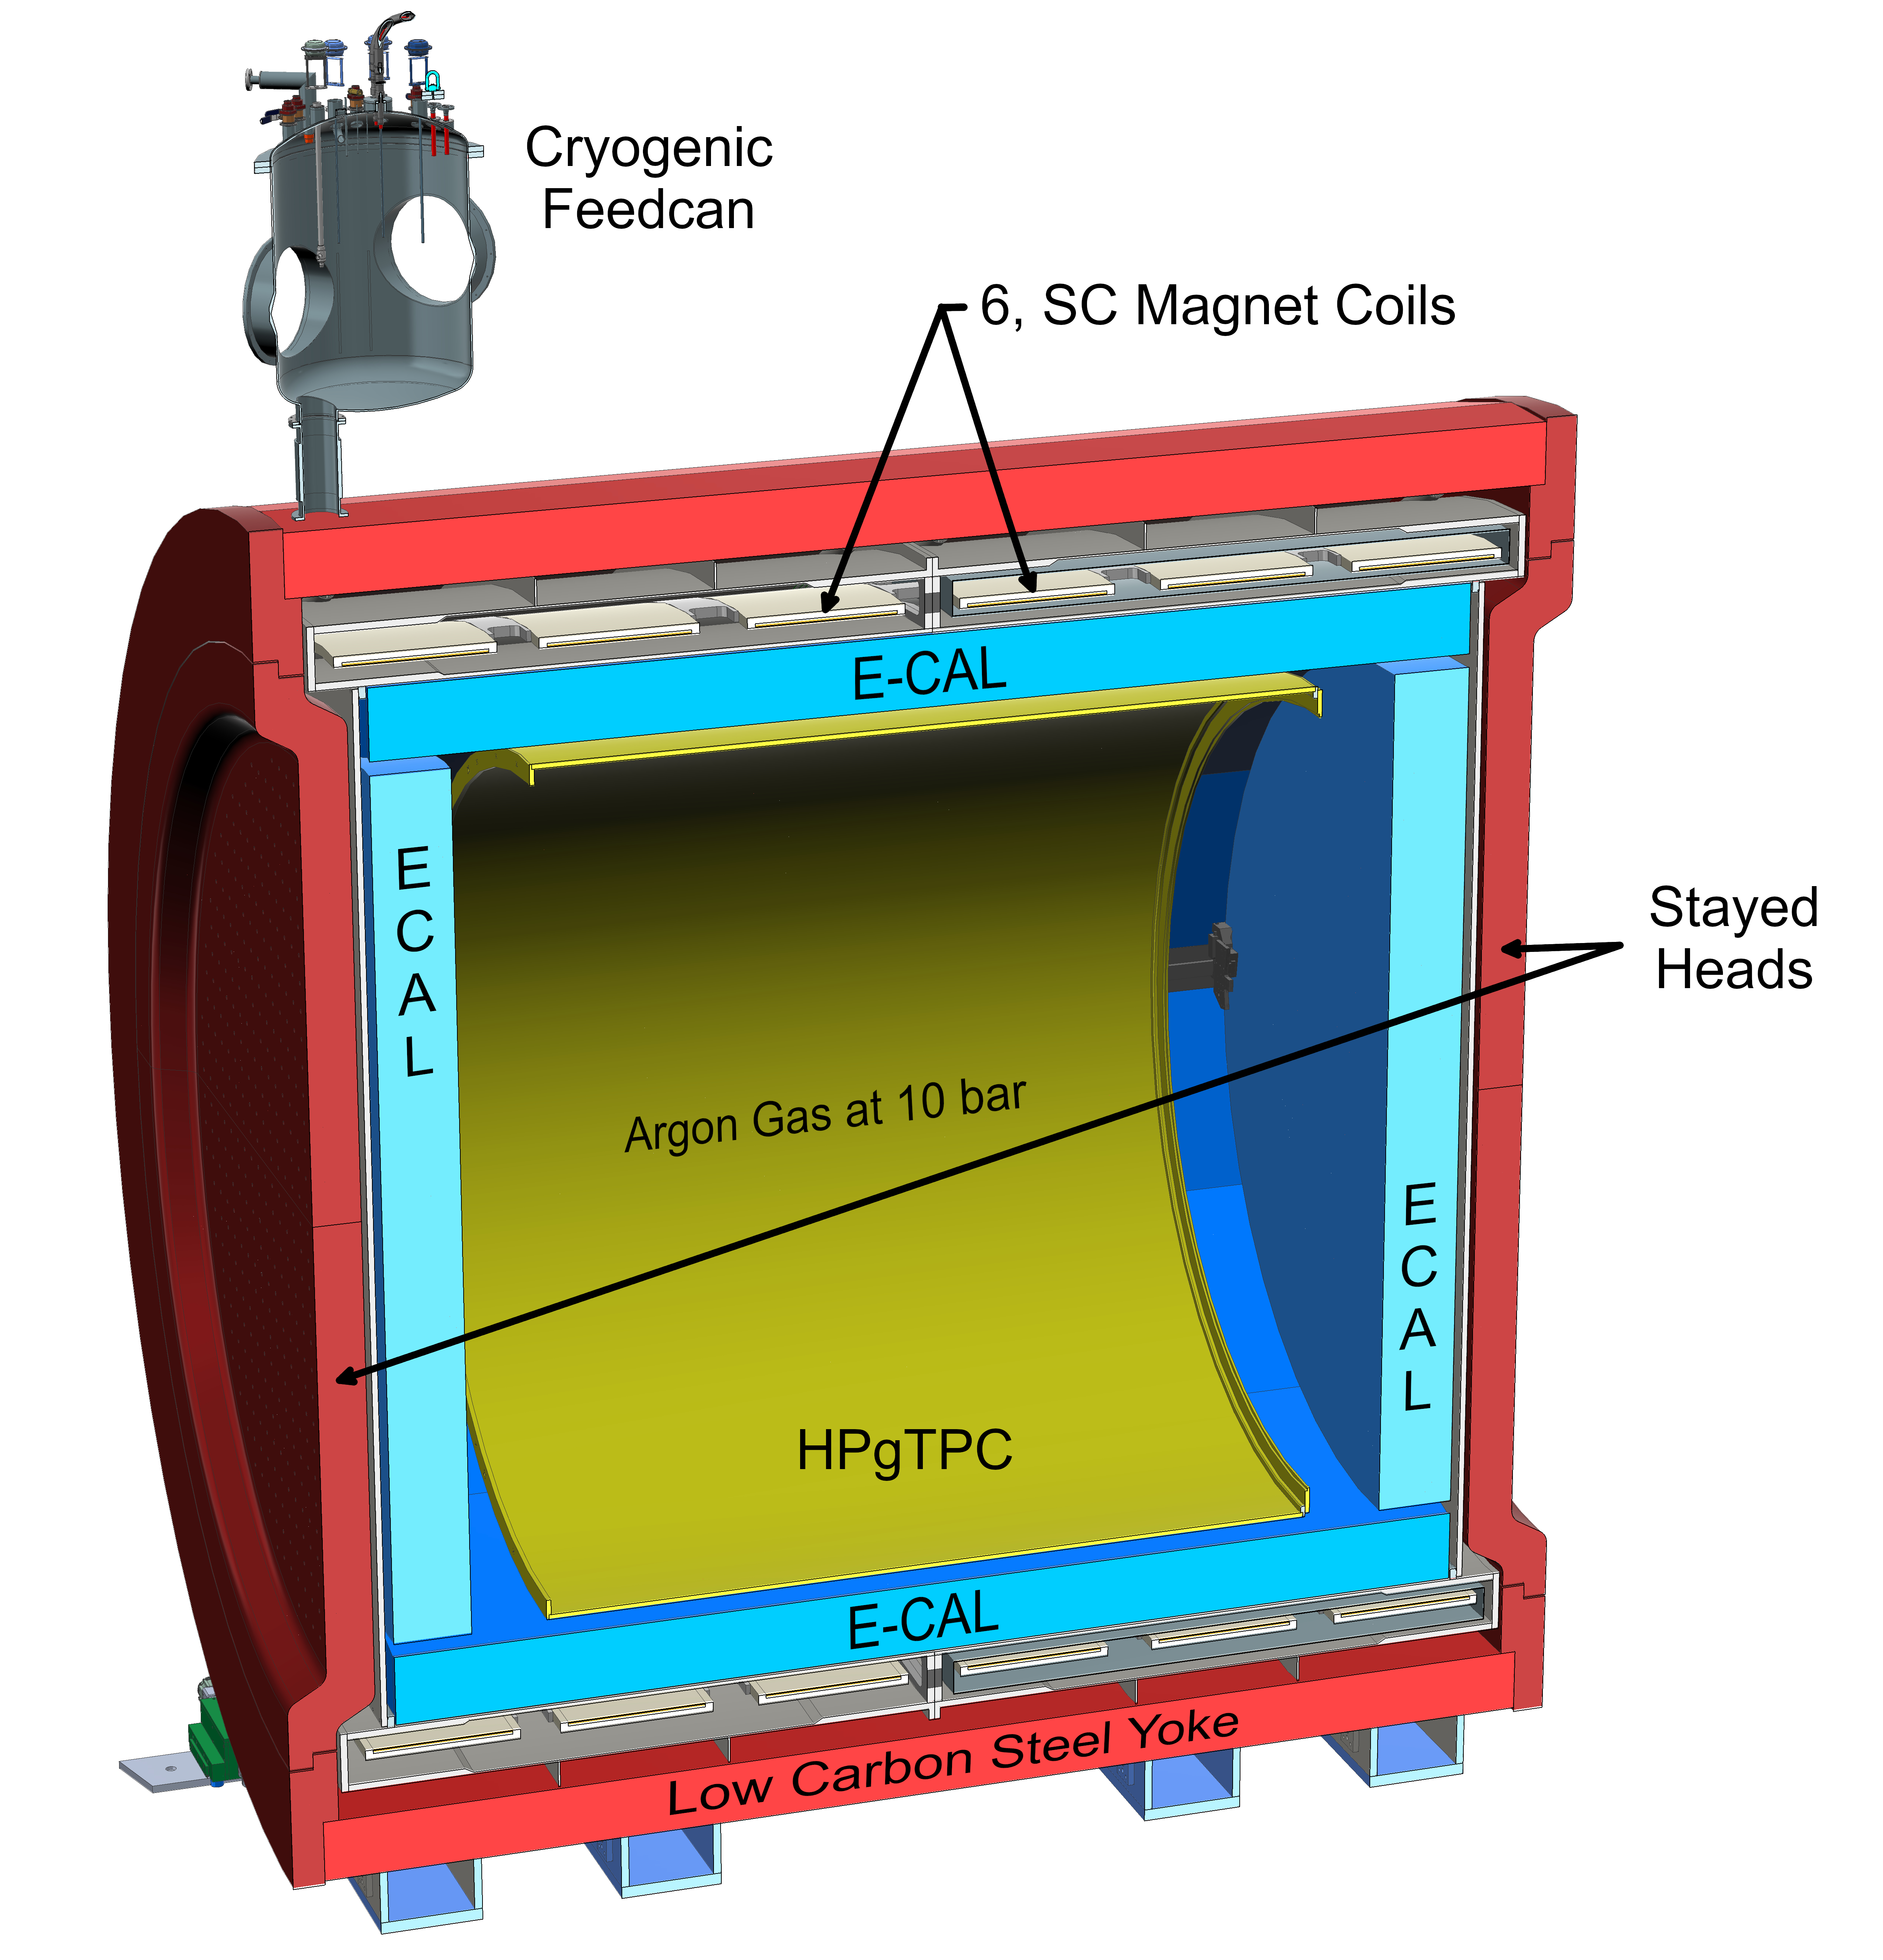
\includegraphics[width=\textwidth]{figures/ch3-DUNE/SPY_X-section2.jpg}
%          \caption{}
%          \label{fig:ND-G-threshold}
%      \end{subfigure}
%         \caption{(a) Schematic view of the external components of ND-GAr with a cutaway showing the magnet, electro-magnetic calorimeter and the internal TPC  (b) Plot showing proton range in cm as a function of Kinetic Energy in MeV in double logarithmic scale. The different curves show the range dependency in different gaseous, liquid or solid media \cite{Lu}. }
%         \label{fig:GAr}
% \end{figure}

\begin{figure}[t]
     \centering
     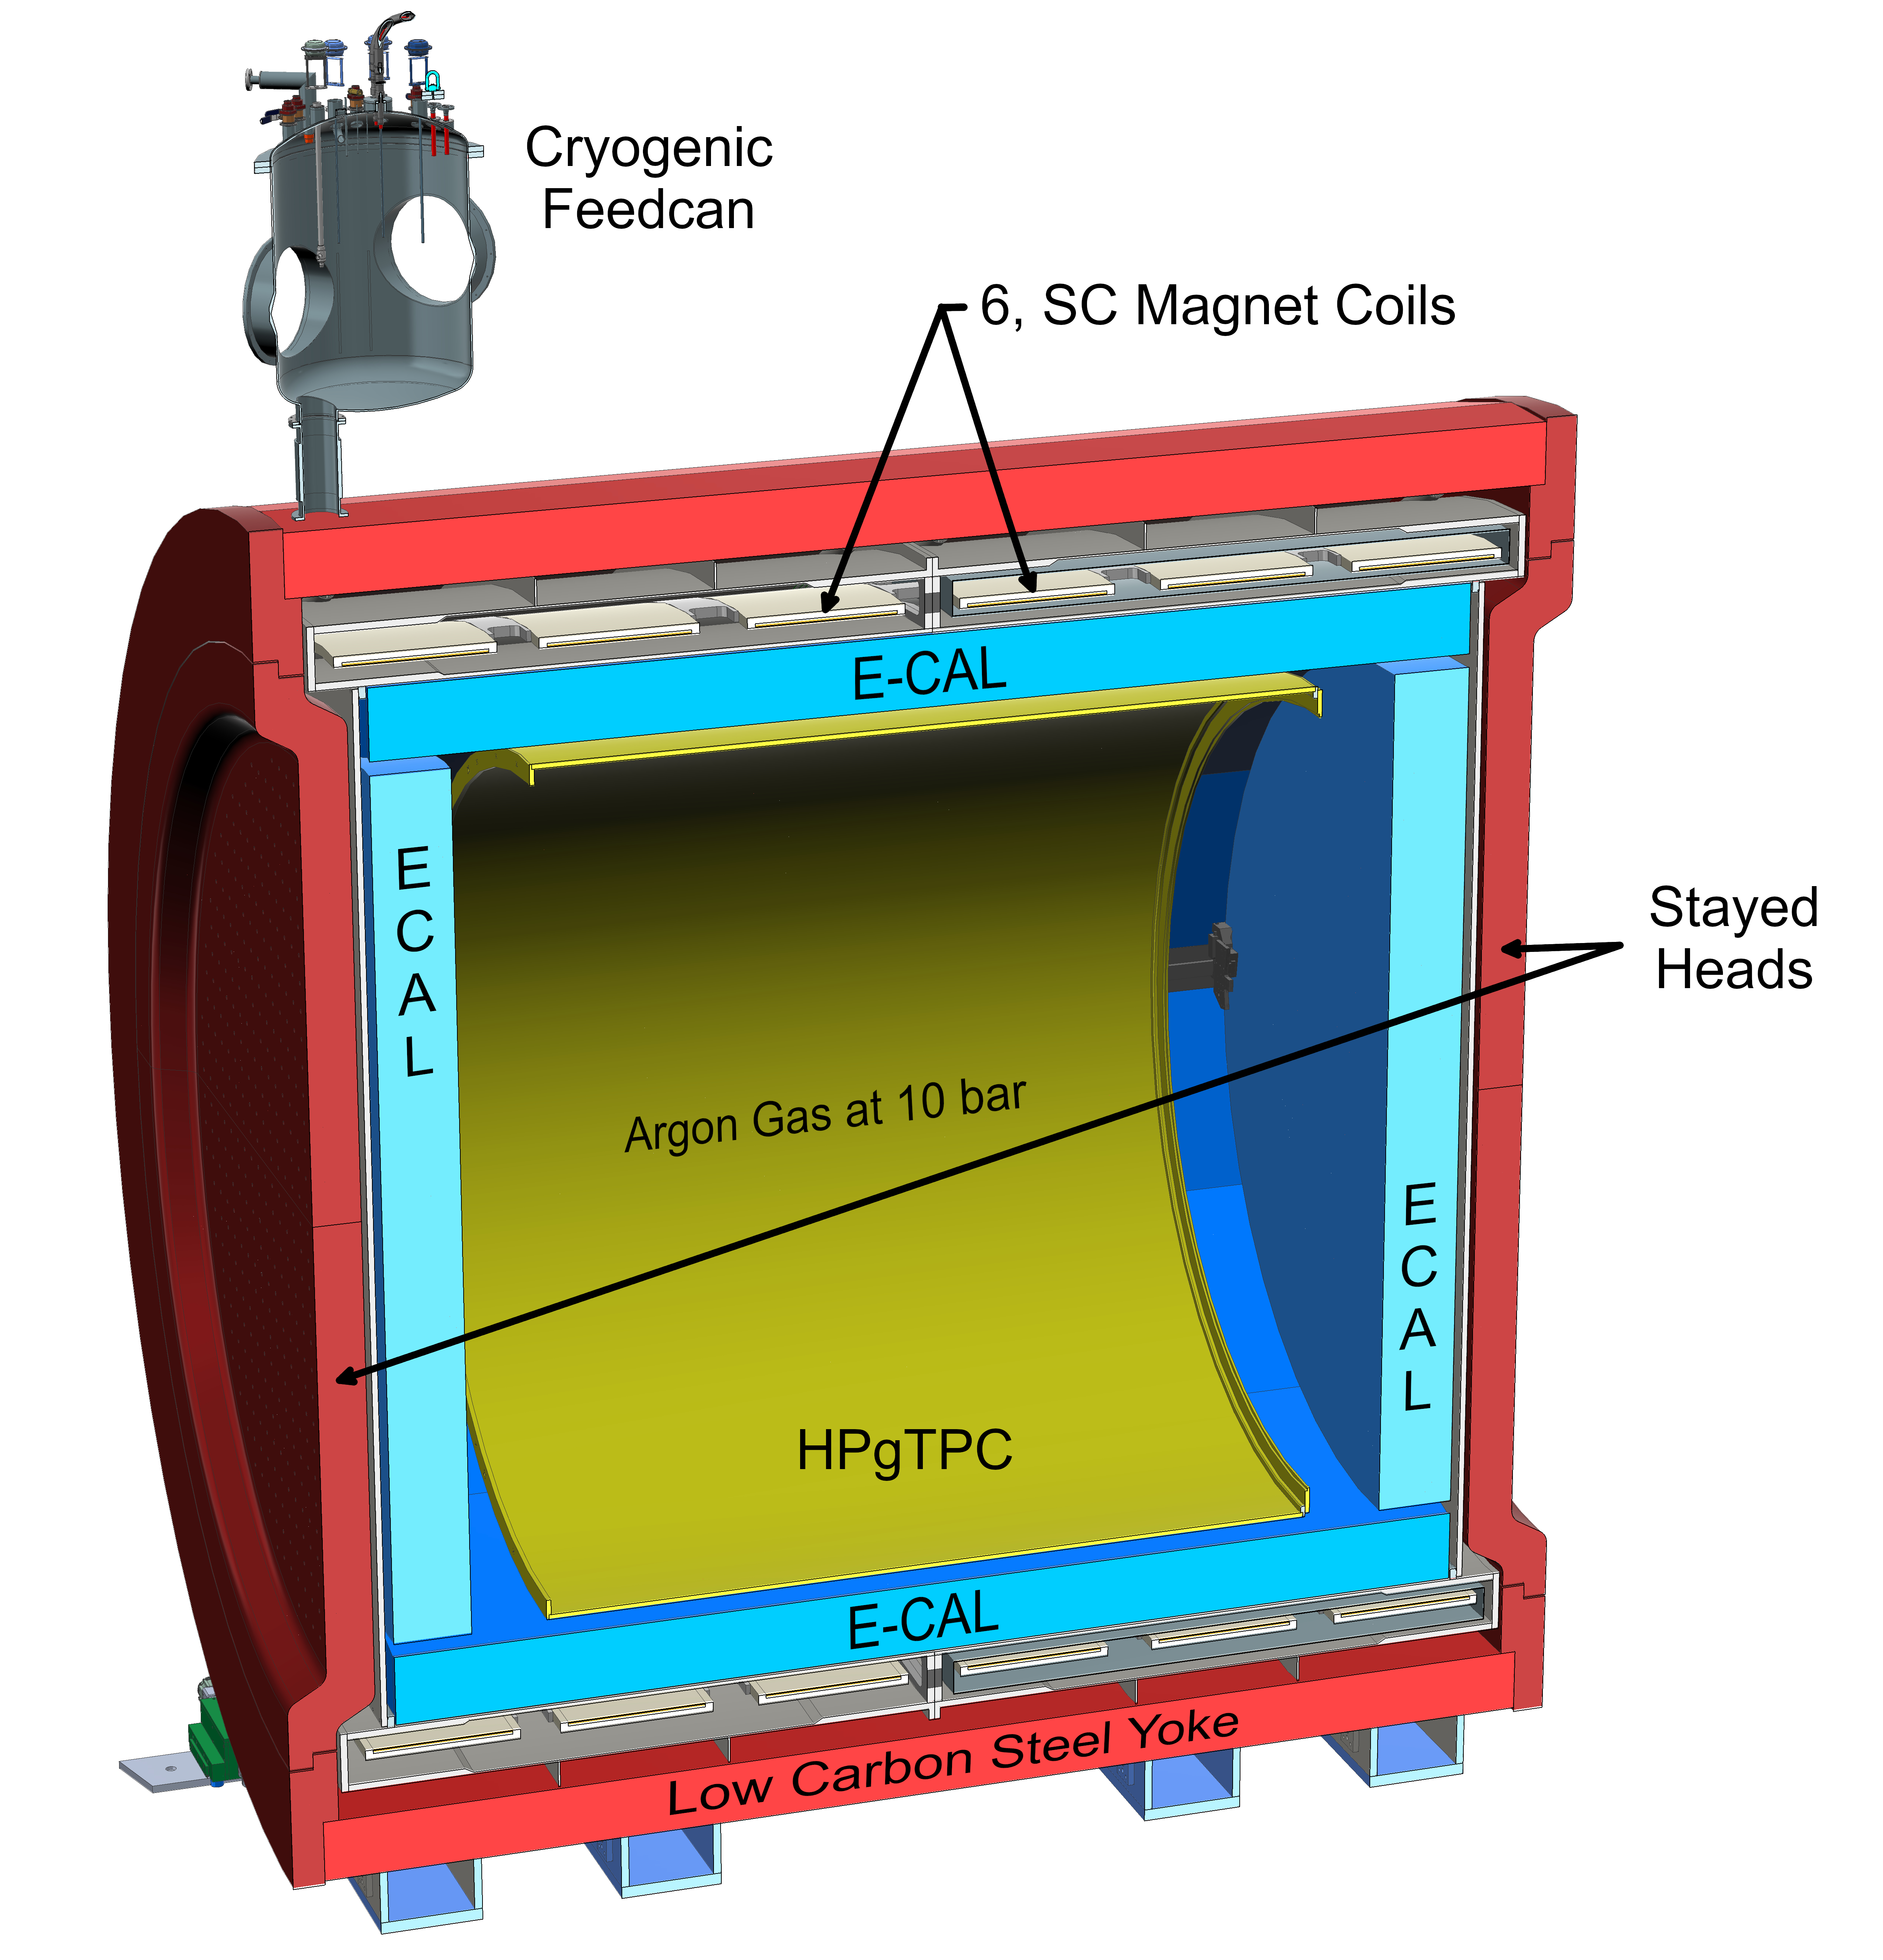
\includegraphics[width=0.6\textwidth]{figures/ch3-DUNE/SPY_X-section2.jpg}
     \caption{Schematic representation of ND-GAr experiment with its main components}
        \label{fig:ND-G}
\end{figure}

ND-GAr will be a magnetized detector with a magnetic field of 0.5T, mainly constituted of a high pressure gas time projection chamber (HPgTPC) surrounded by an electro-magnetic calorimeter (ECAL). A simple cut-away schematic of the detector is shown in Figure \ref{fig:ND-G}. ND-GAr will fulfill two main goals: firstly it will act as a spectrometer measuring the charge and momentum of particles exiting ND-LAr; secondly it will offer its own sample of neutrino interactions inside the HPgTPC. The high pressure gas environment will offer relatively low tracking thresholds and enhanced particle identification (PID) performance when compared to LArTPC's, especially for pion-proton separation. The PID capabilities of ND-GAr specifically derive from a combination of $dE/dx$ measurements in the HPgTPC, $E/p$ measurements in the ECAL and the curvature momentum and sign selection measurements available from the magnetization of the TPC alongside range measurements in the ECAL.

ND-GAr's spectrometer role mostly consists in identifying the sign and measuring the momentum of muons exciting ND-LAr. This is done to measure the spectrum of $\nu_\mu$ and $\Bar{\nu}_\mu$ reaching the near detector, through their CC interaction products. This is crucial to reach the oscillation measurement sensitivity desired by the experiment.

\begin{figure}[t]
     \centering
     \includegraphics[width=0.7\textwidth]{figures/ch3-DUNE/threshold.png}
     \caption{Schematic representation of ND-GAr experiment with its main components}
        \label{fig:ND-G-threshold}
\end{figure}

ND-GAr's lower tracking thresholds as well as its superior PID capabilities and acceptance, will make kinematic regions not accessible to a LAr detector, available to the ND complex. The relationship between proton tracking threshold and tracking material can be seen in Figure \ref{fig:ND-G-threshold}. This is particularly important to enhance the ability of the ND of clarifying the relationship between the true and reconstructed energy in neutrino interactions on Argon. Nuclear effects such as final state interactions (FSI), Fermi motion and 2p2h effects can introduce significant systematic uncertainties in the reconstruction of the neutrino energy. Theoretical studies suggest for example that FSI can increase dramatically the number of final state protons in the kinetic range of 10s of MeV's and it's thus crutial for the ND to be able to measure them and identify them. This is possible with a HpGTPC which has lower tracking thresholds, but not in a LAr or solid detector such as ND-LAr or SAND. 

It is also important for ND-GAr to characterize the spectrum of charged pions coming from $\nu_\mu$ and $\Bar{\nu}_\mu$ CC interactions. At very low energies, down to 20 MeV , this is essential because this is the region where FSI's are more prevalent. Only a gaseous detector has low enough energy thresholds to do it with a sufficient efficiency. At higher energies above 100 MeV, ND-GAr becomes essential in distinguishing the pion multiplicity, since in LAr the same pions tend to produce hadronic showers, while in ND-Gar's TPC they are more likely to  produce distinguishable tracks. Measuring neutral pions from $\nu_\mu$ and $\Bar{\nu}_\mu$ CC interactions in the same momentum range is also possible for ND-GAr thanks to its ECAL.

\subsection{The HpGTPC}
The design of ND-GAr's HPgTPC is closely related to the design of the ALICE experiment's TPC \cite{ALICE}. The basic detection mechanisms of ALICE's and ND-GAr's TPC's are identical. The primary ionization electrons are formed by the energy deposition of passing charged particles, and drifted towards the end-caps by a an electric field produced by a high voltage (HV) central electrode plane. The total drift region has a cylindrical shape with a diameter of $\sim 5m$ and a length of $\sim 5m$ and the electric field is oriented in parallel to the 0.5T magnetic field, in order to reduce transverse diffusion. At the end-caps, multi-wire proportional chambers (MWPC's) induce electron avalanches which produce a signal on an anode pad plane. Read-outs of the pad signals give hit coordinates in two dimensions, while the drift time provides the third.

The read-out chambers or ROC's used in ALICE, contain the MWPC's and read-out pad planes and are divided in 18 trapezoidal regions, each including a smaller inner chamber (IROC) and an outer chamber (OROC). All of ALICE's ROC's will be re-installed in ND-GAr, as they have been replaced in the original detector by GEM-based ROC's \cite{Ferretti:2022yjd}. An additional central region of ROC's (CROC's) will fill the central regions of the read-out planes, which in ALICE was occupied by a silicon based central tracker and an inner field cage. 

Despite all the common elements, some key differences between the design of the two TPC's exist: the two detectors will use different gases, with ALICE's base gas being a mixture Ne/CO$_2$/N$_2$ and ND-GAr using a mixture of Ar-CH$_4$ at 90\%-10\% molar fractions; ND-GAr will operate at a pressure 10 times larger than ALICE; the electronics and data acquisition systems will be completely re-designed to be closer to the LArPix technologies used in DUNE's LArTPC's; the field cage will only include an outer component, since the central region in ND-GAr will be part of the active volume of the detector, while in ALICE it was occupied by the the beam pipe and a silicon-based tracker.
\begin{figure}[t]
     \centering
     \begin{subfigure}[b]{0.52\textwidth}
         \centering
         \includegraphics[width=\textwidth]{figures/ch3-DUNE/ALICE_TPC_dEdx_Lippmann_2012.png}
         \caption{}
         \label{fig:ALICEPID}
     \end{subfigure}
     \hfill
     \begin{subfigure}[b]{0.47\textwidth}
         \centering
         \includegraphics[width=\textwidth]{figures/ch3-DUNE/PEP4-TPC-80Ar-20CH4-8_5atm_dEdx.png}
         \caption{}
         \label{fig:PEPPID}
     \end{subfigure}
        \caption{(a) Schematic view of the external components of ND-GAr with a cutaway showing the magnet, electro-magnetic calorimeter and the internal TPC  (b) Plot showing proton range in cm as a function of Kinetic Energy in MeV in double logarithmic scale. The different curves show the range dependency in different gaseous, liquid or solid media \cite{Lu}. }
        \label{fig:PID}
\end{figure}

The HPgTPC is oriented so that the neutrino beam is perpendicular to the electric and magnetic fields. This is the most favorable orientation for measuring charged particles traveling along the neutrino beam direction. In ALICE the track reconstruction is done by combing ROC hits to form tracks following the trajectories of charged particles in the TPC. This is done for ND-GAr through the GArSoft software package which handles the simulation and reconstruction for the detector. A comprehensive description of this tool will be given later in Sec. and Sec. respectively. 

In ALICE the ionization induced by charged particle tracks can be used to estimate the particle's $dE/dx$. When combined with a curvature momentum estimate, this can be used for PID. In Fig. \ref{fig:ALICEPID} we show the characteristic PID curves for charged particles produced in proton-proton collisions at $\sqrt{s}=7 \textrm{TeV}$. The band resolution of the different particle types $dE/dx$ curves is expected to be significantly improved in ND-GAr. The 10 times higher gas pressure in ND-GAr will result in a correspondend increase in ionization per unit track length. A better comparison can thus be made with the performance of the PID capabilities of PEP-4/9, which operated at 8.5 atmospheres: the experiment's $dE/dx$ curves are plotted in Fig. \ref{fig:PEPPID} showing good separation between particle types below a few GeV, including pions and muons which are problematic for lower material budget TPC's. 

\begin{figure}[t]
     \centering
     \begin{subfigure}[b]{0.7\textwidth}
         \centering
         \includegraphics[width=\textwidth]{figures/ch3-DUNE/dpmuon.pdf}
         \caption{}
         \label{fig:GArTPCdp}
     \end{subfigure}
     \hfill
     \begin{subfigure}[b]{0.7\textwidth}
         \centering
         \includegraphics[width=\textwidth]{figures/ch3-DUNE/muonpoverpfunc.pdf}
         \caption{}
         \label{fig:GArTPCdpoverp}
     \end{subfigure}
        \caption{(a) Schematic view of the external components of ND-GAr with a cutaway showing the magnet, electro-magnetic calorimeter and the internal TPC  (b) Plot showing proton range in cm as a function of Kinetic Energy in MeV in double logarithmic scale. The different curves show the range dependency in different gaseous, liquid or solid media \cite{Lu}. }
        \label{fig:GARTPCdp}
\end{figure}

The resolution of a curvature momentum measurement in a TPC depends on the pad resolution as well as the multiple coulomb scattering (MS) degradation (see Sec for a more in depth discussion). The characteristics of the track and of the neutrino event also influence the curvature resolution. These include the particle's transverse momentum $p_T$ the track's length as well as the detector's occupancy at the time of the track formation.

Given the randomized nature of particle track formation in a neutrino experiment, the distribution of the tracks length is expected to have a significant component of short tracks. For this reason fiducial cuts are imposed inside the TPC. Note that low energy particles that stop within the detector (primarily protons) would be reconstructed via their track length rather than their curvature. Within the fiducial volume ND-GAr will have a $4\pi$ acceptance. This include particles crossing the central cathode region, which is very thin (25 $\mu m$ of mylar).

An early study was done using the GArSoft software suite, on the momentum resolution for muons coming from $\nu_\mu CC$ interactions in the HpGTPC using the LBNF flux. A fiducial cut was imposed on the interaction vertexes requiring a distance of at least 50 cm from the barrel walls and 30 cm from the end-caps. The momentum resolution was calculated in terms of fractional residuals defined as:
    \begin{equation}
        \frac{\Delta p}{p_\textrm{true}} = \frac{p_\textrm{reco}-p_\textrm{true}}{p_\textrm{true}}
    \end{equation}
where $p_\textrm{true}$ is the true initial momentum of the particle while $p_\textrm{reco}$ is the reconstructed one. The distribution was fitted with a double Gaussian function defining a "core" and a tails resolution. The resolution defined by the $\sigma$ of the residual distribution is of 2.7\% for the core distribution and 12\% for the tails as shown in Fig. \ref{fig:GArTPCdp}. The single Gaussian resolution is shown as a function of the muon track length in Fig. \ref{fig:GArTPCdpoverp}.

\subsection{The electro-magnetic calorimeter}
The main role of the ECAL will be to reconstruct electrons and photons coming from neutrino interactions. The ability of detecting photons and identifying their production point makes the reconstruction of $\pi_0$ from inside the HpGTPC possible. This will be especially important in the reconstruction of $\nu_e$ events for which the missed identification of $\pi_0$ produces important systematic uncertainties. The ECAL will also be important in determining the $t_0$ for particles coming from ND-LAr and rejecting external background such as rock muons and neutrons. It will offer a time precision at the sub-nanosecond level.

The reference design of the ECAL is heavily inspired by the CALICE hadron calorimeter from the ALICE experiment \cite{CALICE:2010fpb} as well as the ECAL of the ND280 modules at T2K \cite{T2KUK:2013wkh}. It will have an octagon shape fully contained in the pressure vessel, with each octant composed by trapezoidal modules. The modules will contain alternating layers of active polystirene scintillator read out by SiPm's and absorber sheets. The active layers are segmented in tiles and strip offering an effective space resolution of the order of a few cm's.

\begin{figure}[t]
     \centering
     \includegraphics[width=0.6\textwidth]{figures/ch3-DUNE/Spy.jpg}
     \caption{Schematic representation of ND-GAr experiment with its main components}
        \label{fig:Spy}
\end{figure}

\subsection{The SPY magnet system}
The current integrated design for ND-GAr's solenoid, pressure vessel and yoke is named the Solenoid with Partial return Yoke (SPY) \cite{Bersani:2023rlw} and is largely based on the magnet system developed for the Multi Purpose Detector (MPD) at the NICA Collider at JINR \cite{Golovatyuk:2016zps}. The magnet system is composed of a superconducting magnet surrounded by an iron return yoke. To reduce dimensions and overall costs, the magnet and cryostat system has been designed to serve as the cylindrical component of the pressure vessel for the HpGTPC, while also providing support for the HpGTPC and the ECAL, which will be fully contained inside its volume.

The magnet coil is composed of rectangular superconducting cables bent and grouped to form six identical sub-coils with an internal diameter of 7 m, a length of 0.9m and a thickness of 20 mm, operating at 5000A. The coils will be hosted in a cryostat reaching operating temperatures of 4.5 K to 4.7 K. The cooling elements of the cryostat will consist of pipes welded onto the outer surface of the coil formers hosting a thermosiphon-driven flow of liquid helium. 

SPY's magnet will produce an overall magnetic field of 0.5T with a field uniformity of $\pm 1\%$. These field characteristics surpass the requirements necessary to achieve the particle reconstruction performance desired by ND-GAr. These include a minimum 3\% momentum resolution for muons exiting from ND-LAr and a performance at least as good as the Far Detector for particles produced in neutrino interactions on gas. The yoke has also been designed to reduce the amount of material between ND-LAr and ND-GAr to a minimum by removing a portion of the downstream barrel. This is important to ensure that the muons coming from ND-LAr loose as little energy as possible in un-instrumented portions of the detectors, reducing the relative uncertainties to a minimum.

SPY is completed by a carbon steel return yoke, which presents several unique characteristics. The pole faces of the yoke have been designed to offer sufficient mechanical strength to act also as the end-caps of the detector's pressure vessel. This removes the necessity for the large domed heads that would normally be required for a pressure vessel of such a diameter, shortening the overall dimensions of the system by about 4m.

\section{The temporary muon spectrometer}
\subsection{TMS}
\begin{figure}[t]
     \centering
     \includegraphics[width=0.6\textwidth]{figures/ch3-DUNE/TMS.png}
     \caption{Schematic representation of ND-GAr experiment with its main components}
        \label{fig:TMS}
\end{figure}
The temporary muon spectrometer (TMS) is a magnetized steel range stack detector which is set to become operative during DUNE Phase I. Its main role will be to measure the momentum and charge of muons exiting ND-LAr. This will increase the acceptance of ND-LAr making the performance of the two combined detectors comparable to that of the FD.

Both the Argon Target and the technology of ND-LAr are essential to predict the rate and spectrum of neutrino-argon interactions expected at the FD and achieve the level of control over the systematics necessary for the Phase I physics goals. The inclusion of a magnetized muon catcher to ND-LAr is important to improve the muon momentum reconstruction performance in the key energy range between 0.5 and 5 GeV reaching a resolution of the order of $\delta p / p \sim 5\%$. The sign selection, which is not available using ND-LAr alone, is crucial in the $\delta_\textrm{CP}$ measurement. This is especially true in reverse horn current where the beam will experience a large contamination of neutrino interactions comparable to the desired anti-neutrino interactions. In measuring $\Bar{\nu}_e$ appearance, the sample of $\nu_e$ interactions needs to be carefully accounted for.

TMS consists of 100 alternating layers of magnetized steel absorber and plastic scintillator. A schematic representation of the detector is shown in Fig. \ref{fig:TMS} . Each scintillator layer consists of four panels divided into 48 strips, all 300 cm long and 3.5 cm wide. The strips in each layer are tilted in an alternating pattern by $\pm 3^\circ$ with respect to the vertical direction, providing U and V views. Each layer of steel will divided into three colums, each magnetized by two electrified coils. The coils which surround the central block produce a magnetic field which faces downwards, while the two later blocks have a magnetic field pointing  in the opposite direction. The thickness of the steel plates is of 15 mm for the first 40 layers upstream and of 40 mm in all the others. The thickness of the steel layers was chosen in order to optimize the particles' energy deposition.

In TMS the muon momentum will be measured by range, while the charge sign will be determined based on the curvature of the particle trajectory. The scintillator layers are instrumented with ADC's and can provide calorimetric information as well as position measurements. This information can be used in many ways: the Bragg peak can be identified to identify stopping muons more effectively; muons experiencing very high energy loss via bremmstrahlung can be selected and more effectively reconstructed; the stopping point can be more effectively found by studying the evolution of $1/\beta^2$ along the track. Calorimetric measurements of muon energy can also be made but they are not expected to be competitive with the range measurements. 

The capabilities of TMS will be sufficient to reach the physics goals of the DUNE collaboration during Phase I, where the uncertainties will be dominated by the lack of statistics. This won't be true for Phase II where the impact of the systematics will be much larger. This is why TMS will be substituted by a more capable Near Detector (MCND) module, the leading design currently corresponding to ND-GAr. 

\subsection{ND-GAr-Lite}
\label{Sec: DUNE-GArLite}

ND-GAr was an alternative Phase I muon spectrometer design for the ND which would have become possible in the case that early funds for the construction of the SPY magnet system had become available (see Fig. \ref{fig:Lite} for a schematic representation of the design). The detector would have included all the components of the SPY system while the central volume of the magnet would have been instrumental with a minimal amount of Minerva-inspired scintillator tracking planes. The advantage of this approach was to provide a natural staging to the construction of ND-GAr, reducing overall cost and wastes compared to the TMS design which is set to be fully removed from the ND in the transition between Phase I and II. The ND-GAr-Lite design was eventually abandoned by the collaboration as it became clear that the funds necessary to build the SPY magnet were not going to be available for Phase I. 

Two plans were originally envisioned for the transition between ND-GAr and ND-GAr-Lite. The first approach was the most straightforward and consisted in building the ECAL and HpGTPC above ground and lowering them in the ND chamber at the same time. They would have been then mounted inside the already functioning spy magnet and enclosed inside the pressure vessel. The estimated shut-down for such a scenario would have been of the order of 8 months, similar to the 6 months estimated for TMS. The second plan consisted in a staged approach where the ECAL would have been inserted first, while keeping the tracking planes in place. The HpGTPC would have been inserted soon after completing the design. This staged approach had the potential to reduce beam shut-down to a minimum but was never fully studied.

\begin{figure}[t]
     \centering
     \includegraphics[width=0.8\textwidth]{figures/ch3-DUNE/MPD_Magnet_w_Tracker_Planes.jpg}
     \caption{Schematic representation of ND-GAr-Lite experiment with its main components}
        \label{fig:Lite}
\end{figure}

The nominal design for ND-GAr-Lite’s tracker consisted of a series of rectangular tracking stations, all roughly 5.8m tall and 5.1m tall, positioned perpendicularly to the beam direction.
Each plane would have included a x-plane and a y-plane composed of triangularly shaped scintillator bars, approximately 4cm wide and 2 cm tall. Each bar would be equipped with a detector module
called quad-counter, which would include a motherboard reading out 4 SiPMs which in turn would detect the light from 4 wavelength-shifting fibers. 

An additional muon tagger plane to be placed between ND-LAr and ND-GAr-Lite was also considered by the collaboration. This muon-tagging system would not have been removed in the transition between Phase I and II and would have been especially useful to ND-GAr for $\mu/\pi$ separation. A muon-tagging system is still being considered by the collaboration but no mature design exists.  

% \begin{figure}[t]
%      \centering
%      \includegraphics[width=0.7\textwidth]{figures/ch3-DUNE/6plane.png}
%      \caption{Schematic representation of ND-GAr-Lite experiment with its main components}
%         \label{fig:Lite6}
% \end{figure}

In order to form a track, ND-GAr-Lite requires at least three hits in three unique planes. The nominal tracker design included 5 planes, placed symmetrically about the center of the internal cylinder of the detector. This configuration was eventually substituted by a new design which used 6 unequal planes, mostly placed in the upstream half of the ND-GAr cryostat. The nominal design had a tracking momentum threshold for muons exiting ND-LAr of 1 GeV/c and an angular acceptance of $\sim$ 20 deg. The new arrangement extended the tracking capability to cover nearly all of the muon kinematic phase space, improved the overall tracking efficiency, and lowered the threshold to track muons with initial momenta as low as 700 MeV/c.

For both detector configurations the relative momentum resolution for ND-LAr generated muons was studied and oscillated between 2\% and 4\% over a wide range of momenta. These results satisfied the $\leq 4\%$ ND requirements for a Phase I muon spectrometer.  

\section{Dune's scientific program}
\subsection{Neutrino oscillation measurements}
The central aim of DUNE is to challenge the three-flavour neutrino oscillation paradigm at an unprecedented level of precision. It will do this by performing neutrino oscillation parameter measurements which will allow to shed light on key questions in the field. The neutrino mass ordering remains undetermined with current measurement only marginally preferring the normal hierarchy hypothesis.  The value of $\delta_\textrm{CP}$ is poorly constrained with all possible values in the range between $\pi$ and $2\pi$ being consistent with data. Finally the value of $\theta_{23}$ is known to be close to the maximal mixing value $\pi/4$ but its octant is still unresolved. DUNE aims to provide answers to all these unopened questions.

In long-baseline experiments such as DUNE that have access to horn-focused beams producing either $\nu_\mu$ or $\bar{\nu}_\mu$ dominant fluxes, the oscillation parameters can be studied either through disappearance or appearance measurements. While due to the almost maximal value of $\theta_{23}$ the $\nu_\mu\rightarrow\nu_\tau$ is the dominant one, it can only be studied indirectly through disappearance. This is due to the fact that the oscillation maxima occur at energies below the threshold for $\tau$-lepton production in $\nu_\tau \ CC$ interactions. On the other hand the sub-dominant channel $\nu_\mu\rightarrow\nu_e$ allows for the detailed study of many oscillation properties through the measurement of of energy dependent $\nu_e$ and $\bar{\nu}_e$.

If we assume a constant matter density the oscillation probability $\nu_\mu\rightarrow\nu_e$ can be written as:
\begin{equation} \label{eq1}
    \begin{split}
        P(\nu_\mu\rightarrow\nu_e) & = \sin^2\theta_{23} \sin^22\theta_{13} \frac{\sin^22(\Delta_{31}-aL)}{(\Delta_{31}-aL)^2}\Delta_{31}^2\\
         &  +\sin2\theta_{23} \sin2\theta_{13} \sin2\theta_{12} \frac{\sin^22(\Delta_{31}-aL)}{(\Delta_{31}-aL)}\Delta_{31}\\
         & \times\frac{\sin(aL)}{(aL)}\Delta_{21} \cos(\Delta_{31}+\delta_\textrm{CP})\\
         & +\cos^2\theta_{23} \sin^22\theta_{12} \frac{\sin(aL)}{(aL)}\Delta_{21} \Delta_{21}^2
    \end{split}
\end{equation}
where $\Delta_{ij}=\Delta m_{ij}^2L/4E_\nu$, $a = G_FN_e\sqrt{2}$, $G_F$ is the Fermi constant, $N_e$ is the number density of electrons in the Earth, $L$ is the baseline in km, and $E_\nu$ is the neutrino energy in GeV. In the
equation above, both $\delta_\textrm{CP}$ and $a$ switch signs going from the $\nu_\mu\rightarrow\nu_e$ to the $\bar{\nu}_\mu\rightarrow\Bar{\nu}_e$ channel which implies that a neutrino-antineutrino asymmetry is introduced both by CPV ($\delta_\textrm{CP}$) and the matter effect ($a$). As explained in Sec. [ref] the matter effect asymmetry simply arises from the presence of electrons in the Earth's matter, with which $\nu_e$'s have a high probability to interact and $\bar{\nu}_e$ do not. In the few GeV range the interaction probability of $\nu_e$'s and thus the  impact of matter effect increase with the amount of matter traversed by the neutrino. Experiments with longer baselines are thus more sensitive to matter effects and consequently to the mass ordering. DUNE, with its 1300km baseline, will be able to resolve the degeneracy between the matter and CP-violating asymmetry and determine both the neutrino mass ordering and the value of $\delta_\text{CP}$ at $5\sigma$ for more than 50\% of its possible true values \cite{Diwan:2004bt}.

The measurement of $\delta_\text{CP}$ in DUNE also benefits from the use of a wide-band neutrino beam. In Fig. \ref{fig:energy_nu} we show the $P(\nu_\mu\rightarrow\nu_e)$ as a function of neutrino energy at a 1300 Km baseline for three maximal values of $\delta_\text{CP}=-\frac{\pi}{2},0,\frac{\pi}{2}$. The various oscillation nodes are clearly visible, with the main one being peaked at 2.4 GeV, where DUNE's neutrino flux will also be peaked. The value of $\delta_\text{CP}$ impacts both the amplitude and the phase of the oscillation nodes, thus being capable of measuring the rate of $\nu_e$ appearance as the function of the neutrino spectrum is highly desirable. In particular the impact of $\delta_\text{CP}$ on the amplitude of the oscillation probability peaks is higher at nodes below neutrino energies of 1.5 GeV, making the ability of DUNE of measuring $\nu_e$ appearance in a wide range, down to at least 500 MeV highly impactful.

While the determination of the neutrino mass hierarchy and the discovery of CP-violation in the leptonic sector will be the main goals of DUNE's oscillation program, the measurements of all the other parameters regulating the oscillation probability will also be a key focus. Particular importance will be given to the measurement of the the mixing angles $\theta_{13}$ and $\theta_{23}$. The $\theta_{13}$  mixing angle has been accurately measured in reactor experiments, which will provide constraint to the DUNE oscillation analysis in the early stages of the experiment. However, to reach the desired levels of systematics constraint, DUNE will have to perform a measurement of $\theta_{13}$ which is independent from and competitive with the reactor results. The measurement in DUNE will be done using a $\nu_e$ and $\bar{\nu}_e$ appearance channel, whereas in reactor experiments it is performed through $\bar{\nu}_e$ disappearance.

\begin{figure}[t]
     \centering
     \begin{subfigure}[b]{0.48\textwidth}
         \centering
         \includegraphics[width=\textwidth]{figures/ch3-DUNE/energy_nu_no.pdf}
         \caption{}
         \label{fig:energy_nu_no}
     \end{subfigure}
     \hfill
     \begin{subfigure}[b]{0.48\textwidth}
         \centering
         \includegraphics[width=\textwidth]{figures/ch3-DUNE/energy_anu_no.pdf}
         \caption{}
         \label{fig:energy_anu_no}
     \end{subfigure}
        \caption{: The appearance probability at a baseline of 1300 km, as a function of neutrino energy, for $\delta_\text{CP}$ (blue), 0 (red), and $\pi/2$ (green), for neutrinos (left) and antineutrinos (right), for normal ordering. The black line indicates the oscillation probability if $\sigma_{13}$ were equal to zero. Note that DUNE will be built at a baseline of 1300 Km \cite{DUNE:2020TDR1}. }
        \label{fig:energy_nu}
\end{figure}


The measurement of $\sin^2\theta_{23}$ in DUNE will help disambiguate its value, potentially pointing to a previously unknown symmetry between the $\nu_2$ and $\nu_3$ mass eigen-states.  Current world measurements are ambiguous on whether the values of $\theta_\text{23}$ lies in the lower octant ($<45^\circ$) or the higher octant ($>45^\circ$) and allow for the maximal value $\sin^2\theta_{23}=0.5$ \cite{Esteban:2018azc}. This would implicate that the $\nu_\tau$ flavor eigen-state receives equal contributions from the mass eigen-states $\nu_2$ and $\nu_3$, which would point towards a previously unknown symmetry. 

Overall obtaining measurements of all the oscillation parameters within a single wide-band oscillation experiment has great value, because it provides a clear observation measurement of the neutrino oscillation pattern allowing for a detailed test of the three-flavor neutrino model. Additionally precise measurements of the PMNS mixing values, allows for comparison with mixing patterns in other areas of the standard model such as quarks. The question of why the quark mixing angles are smaller than the lepton mixing angles remains unanswered and constitutes an important part of the flavor pattern question \cite{King:2014nza}. 


\subsection{Nucleon decay}
\label{Sec:ProtonDecay}
Many beyond the standard model theories theories propose the unification  of the strong, electromagnetic and weak interactions. These Grand Unified Theories (GUTs) extend the standard model introducing a unified gauge symmetry at very high energies ($>10^{15}$ GeV) \cite{deBoer:1994dg}.. One of the key low energy experimentally verifiable predictions that GUT's have in common is nucleon decay \cite{Langacker:1980js}. The dominant modes for proton decays predicted by GUT's are $p\rightarrow K^+ + \bar{\nu}$ and $p\rightarrow K^+ +\pi^0$. The first and second mode are dominant in supersymmetric and non-supersymmetric GUT's respectively. While no evidence of supersymmetry has been found at the electroweak scale, despite extensive efforts at the Large Hadron Collider (LHC), the main appeal of GUT's, which consists in gauge-coupling unification remains intact. 

Many experiments have performed searches of nucleon decay, imposing lifetime limits which already constrain the viability of several GUT models. Currently the best limits on most nucleon decay modes are set by the Super Kamiokande experiment, which features the largest mass and exposure time (more than 30 years) of any detector to date \cite{Super-Kamiokande:2014otb, Super-Kamiokande:2016exg, Super-Kamiokande:2017gev}. Extending the lifetime limits will require detectors to feature long exposure times combined with either large sensitive masses or improved detection efficiency or background rejection. The FD LArTPCs feature all these characteristics. Their excellent imaging, calorimetric and particle identification capabilities, combined with their large liquid argon mass, make them ideal detectors for a nucleon decay search. The LArTPC technology is particularly well suited for the $p\rightarrow K^+ +\bar{\nu}$ or any decay mode that involves charged kaons, because it offers the oppotunity to observe the entire decay chain. In a water Cherenkov detector such as Super Kamiokande the kaons emerging from these decay modes are usually below threshold, but in a LArTPC they can be identified both by their distinctive $dE/dx$ as well as their decay.   Therefore, this mode can be tagged in a LArTPC by looking for single kaons within a suitable  energy range with their point of origin lying within the fiducial volume followed by its decay products. The background induced by cosmic ray muons can be contained imposing fiducial volume cuts and stringent kaon identification requirements. The dominant background is thus produced by atmospheric neutrino interactions.

The DUNE FD will however not limit its search to a single mode or a few dominant channels, but it will be a broad program covering many decays. These efforts are made all the more interesting by the fact that during DUNE's lifetime, two other large detectors, Hyper-Kamiokande \cite{Hyper-Kamiokande:2018ofw} and JUNO \cite{JUNO:2015sjr} are set to perform searches for nucleon decays. If any of the experiments were to observe a signal, having confirmation from other experiments using drastically different detector technologies and thus different backgrounds would be very powerful. 
\subsection{Atmospheric Neutrinos}
\label{Sec:AtmosphericNeutrinos}
\clearpage
\subsection{Supernova neutrinos}
\subsection{Beyond the Standard Model Physics}
\section{Near Detector Physics}
\subsection{Flux and cross section measurements}
\subsection{Beyond the standard model physics and other SM opportunities}
%\subsection{ND-GAr Physics}